% Options for packages loaded elsewhere
\PassOptionsToPackage{unicode}{hyperref}
\PassOptionsToPackage{hyphens}{url}
%
\documentclass[
]{article}
\usepackage{lmodern}
\usepackage{amssymb,amsmath}
\usepackage{ifxetex,ifluatex}
\ifnum 0\ifxetex 1\fi\ifluatex 1\fi=0 % if pdftex
  \usepackage[T1]{fontenc}
  \usepackage[utf8]{inputenc}
  \usepackage{textcomp} % provide euro and other symbols
\else % if luatex or xetex
  \usepackage{unicode-math}
  \defaultfontfeatures{Scale=MatchLowercase}
  \defaultfontfeatures[\rmfamily]{Ligatures=TeX,Scale=1}
\fi
% Use upquote if available, for straight quotes in verbatim environments
\IfFileExists{upquote.sty}{\usepackage{upquote}}{}
\IfFileExists{microtype.sty}{% use microtype if available
  \usepackage[]{microtype}
  \UseMicrotypeSet[protrusion]{basicmath} % disable protrusion for tt fonts
}{}
\makeatletter
\@ifundefined{KOMAClassName}{% if non-KOMA class
  \IfFileExists{parskip.sty}{%
    \usepackage{parskip}
  }{% else
    \setlength{\parindent}{0pt}
    \setlength{\parskip}{6pt plus 2pt minus 1pt}}
}{% if KOMA class
  \KOMAoptions{parskip=half}}
\makeatother
\usepackage{xcolor}
\IfFileExists{xurl.sty}{\usepackage{xurl}}{} % add URL line breaks if available
\IfFileExists{bookmark.sty}{\usepackage{bookmark}}{\usepackage{hyperref}}
\hypersetup{
  hidelinks,
  pdfcreator={LaTeX via pandoc}}
\urlstyle{same} % disable monospaced font for URLs
\usepackage{longtable,booktabs}
% Correct order of tables after \paragraph or \subparagraph
\usepackage{etoolbox}
\makeatletter
\patchcmd\longtable{\par}{\if@noskipsec\mbox{}\fi\par}{}{}
\makeatother
% Allow footnotes in longtable head/foot
\IfFileExists{footnotehyper.sty}{\usepackage{footnotehyper}}{\usepackage{footnote}}
\makesavenoteenv{longtable}
\usepackage{graphicx}
\makeatletter
\def\maxwidth{\ifdim\Gin@nat@width>\linewidth\linewidth\else\Gin@nat@width\fi}
\def\maxheight{\ifdim\Gin@nat@height>\textheight\textheight\else\Gin@nat@height\fi}
\makeatother
% Scale images if necessary, so that they will not overflow the page
% margins by default, and it is still possible to overwrite the defaults
% using explicit options in \includegraphics[width, height, ...]{}
\setkeys{Gin}{width=\maxwidth,height=\maxheight,keepaspectratio}
% Set default figure placement to htbp
\makeatletter
\def\fps@figure{htbp}
\makeatother
\setlength{\emergencystretch}{3em} % prevent overfull lines
\providecommand{\tightlist}{%
  \setlength{\itemsep}{0pt}\setlength{\parskip}{0pt}}
\setcounter{secnumdepth}{-\maxdimen} % remove section numbering

\author{}
\date{}

\begin{document}

\hypertarget{header-n0}{%
\subsection{Abstract}\label{header-n0}}

\hypertarget{header-n2}{%
\section{Einleitung}\label{header-n2}}

In Zeiten von Industrie 4.0 und Digitalisierung werden immer größere
Datenmengen elektronisch gespeichert und verarbeitet. Da bisherige
Speicherungen zumeist ausschließlich in Papierform vorlagen, werden
Systeme benötigt, welche diese in eine digitale Form übersetzten. Das
Deutsche Zentrum für Luft und Raumfahrt entwickelt für Technische
Dokumentationen ein System, welches diese Aufgabe erfüllen soll.

\hypertarget{header-n4}{%
\subsection{Problemstellung und Zielsetzung}\label{header-n4}}

Aufgrund der hohen Vielfältigkeit im Aussehen und Aufbau von Tabellen,
ist es auch mit modernen Algorithmen schwer eine Tabelle zu erkennen und
ihre Daten zu extrahieren. \\
Darauf aufbauend ist das Hauptziel des Projektes die Realisierung eines
Systems zur automatischen Datenerfassung von Tabellen und ihrem Inhalt
mit der Hilfe Maschinellen Lernens.

\hypertarget{header-n6}{%
\subsection{Vorgehen und Aufbau}\label{header-n6}}

Zur Lösung dieser Aufgabe wurde eine Pipeline erstellt in der die
einzelnen Schritte für ein solches System analysiert, entwickelt und
beleuchtet wurden.

Nach einer Definition der Grundlagen in Kapitel 1 wird in Kapitel 2 der
Stand der bestehenden Forschung betrachtet. In Kapitel 3 werden die
Schritte der Pipeline genauer betrachtet welche in Kapitel 4 im
Zusammenhang einer Prototypische Umsetzung beleuchtet werden.\\
Mit Kapitel 5 wird die Arbeit abgeschlossen und ein Ausblick auf
mögliche zukünftige Verbesserungen gegeben.

Die gesamte Entwicklung wurde nach Scrum Prinzipien durchgeführt. Dabei
wurden die einzelnen Experimente in je einem Sprint umgesetzt. Am Ende
eines jeden Sprints wurde das Projekt auf Grundlage der bisherigen
Ergebnisse neu geplant. \\
Durch diese ständige Überprüfung und Anpassung konnte die Pipeline stets
an die neusten Erkentnisse angepasst werden.

\hypertarget{header-n10}{%
\subsection{Das Deutsche Zentrum für Luft- und
Raumfahrt}\label{header-n10}}

Das Deutsches Zentrum für Luft- und Raumfahrt (DLR) ist ein
Forschungszentrum der Bundesrepublik Deutschland. Es umfasst 8700
Mitarbeiter, verteilt auf 28 Standorte in Deutschland, sowie mehrere
Test- und Betriebsanlagen. Es existieren außerdem 4 Standorte in
Brüssel, Paris, Tokyo und Washington DC. Dabei ist das DLR noch in 51
Institute und 150 Großforschungsanlagen aufgeteilt, welche je ihre
eigenen Schwerpunkte setzten.

Das DLR forscht in mehreren Bereichen, darunter Raumfahrt, Luftfahrt
sowie Verkehr und Energie. Ein weiterer Bereich ist der der
Digitalisierung und der Künstlichen Intelligenz. Dabei arbeitet das DLR
eng mit internationalen Partnern zusammen und ist zum Beispiel
verantwortlich für die Überwachung und Planung von Raumlabor Columbus,
einem Multifunktionslabor auf der ISS (International Space Station)
einer bemannten Raumsatiton im Erdorbit.

Am Standort Jena ist das Institut für Datenwissenschaften untergebracht.
Hier werden Lösungen für neue Herausforderungen der Digitalisierungsära
erforscht. Neben den Bereichen Datenmanagment, IT-Sicherheit und Smart
Systems wird hier auch an Bürgerwissenschaften geforscht, welches sich
zum Ziel gesetzt hat die Wissenschaft besser in die Gesellschaft zu
bringen.

\hypertarget{header-n14}{%
\section{Vorbereitung}\label{header-n14}}

Im folgenden werden die technische Grundlagen der Arbeit sowie genutze
Tools und Frameworks vorgestellt.

\hypertarget{header-n16}{%
\subsection{Genutzte Tools und Services}\label{header-n16}}

\hypertarget{header-n17}{%
\subsubsection{Jupyter Notebook}\label{header-n17}}

Zur Durchführung der einzelnen Experimente wurde das Tool Jupyter
Notebook genutzt.\\
Jupyter Notebook ist ein Web basiertes Tool mit dem die Analyse von
Datenbestände vereinfacht wird. Dabei kann Code in Python, C oder Swift
zur Analyse genutzt werden. Die Oberfläche wird dabei wie bei einem
Dokument verwaltet wobei Code in Blöcke getrennt werden kann. Dadurch
können Zwischenergebnisse direkt eingesehen, Blöcke mehrfach berechnet
und die Zwischenergebnisse analysiert werden.

Als Grundlage wurde die COLAB Umgebung der Firma Google genutzt. Hier
werden einzelne virtuelle Umgebungen erstellt welche je ein Notebook
beinhalten. Die virtuellen Umgebungen können dabei je nach Bedarf mehr
oder weniger Rechenleistung bekommen und es können auch eigene Programme
neben dem Notebook installiert werden. Diese Umgebung hat dabei Zugriff
auf leistungsstarke Graphik und Tensor Prozessing Units (TPU und GPU)
welche für den Einsatz mit Neuronalen Netzen optimiert sind.

\hypertarget{header-n20}{%
\subsubsection{Tensorflow}\label{header-n20}}

Tensorflow ist ein Framework zum programmieren von Datenströmen und wird
zur Entwicklung von Neuronalen Netzwerken genutzt. Es ist in C++
geschrieben und kann mit verschiedensten Sprachen genutzt werden. \\
Entwickelt von Google, wird das Framework dort in Forschung und
Produktivbetrieb in zahlreichen Projekten verwendet.

\hypertarget{header-n22}{%
\subsubsection{Keras}\label{header-n22}}

Keras ist eine Deep Learning Library. Sie wurde von zunächst von
François Chollet initiert und später als Kommunity Projekt
weitergeführt. Sie bietet dabei viele nützliche Funktionen um ein
Neuronales Netz zu entwickeln. Seit Tensorflow 1.4 ist Keras dabei auch
Teil des Tensorflow Frameworks und vereinfacht dessen Nutzung.

\hypertarget{header-n24}{%
\subsubsection{OpenCV}\label{header-n24}}

OpenCV ist eine von Willow Garage entwickelte Library welche entzwischen
von Intel gepflegt wird. \\
Geschrieben in Java, Python, C und C++ stellt die Libary dabei
Algorithmen für die Bildverarbeitung und Computer Vision zur verfügung.

\hypertarget{header-n26}{%
\subsubsection{Flask}\label{header-n26}}

Flask ist ein in Python geschriebenes Webframework. Entwickelt von Armin
Ronacher bietet es Funktionen zur Erstellung von Schnittstellen zwischen
Webservern und Webframeworks.

\hypertarget{header-n28}{%
\subsubsection{Python und Swift}\label{header-n28}}

Python ist eine interpretierte Programmiersprache, und wird meistens als
Skriptsprache verwendet. Sie hat eine sehr leicht lesbare Syntax und
kann sehr einfach Fremdcode laden, womit das Schreiben eines schnellen
Skriptes stark vereinfacht wird.\\
Diese Faktoren machen Python zur optimalen Sprache zum Testen von Ideen,
jedoch ist die Sprache nur bedingt für größere Projekte ausgelegt.

Swift ist eine Multiparadimische Compilersprache, welche auf c basiert.
Aufgrund dessen, ist Sie bei größeren Projekten deutlich performanter
als Python, kann jedoch trotzdem Python Librarys einbinden und nutzen.
Es existiert außerdem ein breites Spektrum an Librarys, welches die
Entwicklung von Lösungen stark vereinfacht.

\hypertarget{header-n31}{%
\subsection{TestDaten}\label{header-n31}}

Um die bereits bestehenden Tools, Programme oder Systeme zu testen oder
neu einzurichten werden Testdaten benötigt.

Hierfür stehen einige Datenpools zu Verfügung, welche sich in Umfang und
Aufbau unterscheiden. Dabei wurden Datenblätter von Herstellern von
Raumfahrtkomponenten für DLR und ESA sowie ein Datensatz der Firma IBM
Australia namens PubLayNet genutzt, welche aus mehr als 300.000
Dokumente besteht.

Die Dokumente müssen dabei vor der Nutzung noch manuell vorbereitet und
beispielsweise mit erwarteten Ergebnissen versehen werden. Das PubLayNet
ist bereits mit solchen Ergebnissen versehen, weswegen es sofort genutzt
werden kann.

\hypertarget{header-n35}{%
\subsection{Neuronale Netze}\label{header-n35}}

Ein Künstliches Neuronales Netz (KNN) ist eine Methode zur
Informationsverarbeitung. Dabei wird, nahe dem Vorbild des Gehirns, ein
Netz aus Neuronen erzeugt.\\
Ein Neuron ist dabei ein Object, welches aus einem Input einen Output
erzeugt. Die Ausgabe wird dabei durch eine Aktivierungsfunktion und den
Aufbau des Neurons bestimmt.\\
Das Netz besteht aus mehreren Schichten. Jede Schicht besteht aus
mehreren Neuronen, welche mit den Neuronen der nächsten Schicht
verbunden sind.

\begin{figure}
\centering
\includegraphics{/Users/christian/Library/Mobile Documents/27N4MQEA55~pro~writer/Documents/6-Thesis/DarstellungeineskünstlichenNeurons.png}
\caption{}
\end{figure}

Jede Verknüpfung zwischen den Neuronen, sowie die Neuronen selbst haben
einen Bias welcher eine Gewichtung des entsprechenden Objects darstellt.

Damit dieses Netz nun eine Aufgabe erfüllen kann, wird es trainiert. Das
Netz kann dabei lernen, indem es die Verbindungen zwischen den Neuronen
verändert, die Bias anpasst oder, in bestimmten Netzen, neue Neuronen
erstellt.

Im folgenden wird dies an einem Trainingsprozess betrachtet welcher sich
überwachtes Lernen nennt:\\
Hierbei werden zunächst Testdaten in das entsprechende Netz gegeben und
das Ergebnis mit der gegebenen Lösung verglichen. Auf dieser Grundlage
werden die Bias des Netzes angepasst. Es ist hierbei nicht vorgesehen
den grundlegenden Aufbau des Netzes zu verändern.

Mathematisch lässt sich ein Netz als Gleichung darstellen: \\
\(y_1 + b_1 ∗ y_2 + b_2 ∗ y_3 + . . . + b_{n−1} ∗ y_n = Output\)

y = Neuron\\
b = Bias

Dabei gilt für alle Neuronen: \(y_n = d_n ∗f(x)\)

d = Gewichtung der Zelle\\
f(x) = Aktivierungsfunktion der Zelle

Jeder Wert der Gleichung stellt dabei eine Matrix mit den einzelnen
Werten der jeweiligen Schicht dar. Die Ausgabe wird nun mit dem
erwarteten Ergebnis vergleichen. Aus der entsprechenden Abweichung
lassen sich dabei die Kosten der Funktion berechnen.

Lösung − Output = Kosten

Da die Kosten den Abstand zum gewünschten Ergebnis darstellen ist es
Ziel dieser Endgleichung, die Kosten zu minimieren. Dafür können
Gewichtungen und Bias angepasst werden, wodurch ein Optimierungsproblem
mit \(2n-1\) Unbekannten entsteht. Diese Unbekannten werden nun mit
jedem Training besser und besser an das gewünschte Ziel angepasst.

Für diesen Lernprozess, wird ein Algorithmus namens Backpropagation
genutzt. Dabei geht man, vom Output aus, jede Schicht durch und gibt
jeder Gewichtung eine Richtung, in die Sie sich entwickeln soll. Diese
Richtung wird, je nach Abstand zum Ziel, verstärkt oder verringert so
dass sich das System besser anpassen kann und nicht übers Ziel
hinausschießt.

Die Anpassung kann dabei Offline oder Online geschehen. Bei der Online
Anpassung werden mehrere Beispiele gleichzeitig in ein Netz gegeben und
das Ergebnis aufkumuliert. Somit lernt man für alle Trainingsbeispiele
gleichzeitig. Beim Offline lernen werden alle Trainingsbeispiele
nacheinander genutzt.

Zu Beginn werden alle Gewichtungen und Bias zufällig gesetzt.

Führt man dieses Training nun über alle Testdaten hinweg durch, so
erhält man eine Funktion bzw. ein Modell, welches die Testdaten
möglichst gut lösen kann. Wie dieses Netz dies tut ist größtenteils vom
Zufall bestimmt, die Neuronen können jedoch mit unterschiedlichsten
Zelltypen und Aktivierungsfunktionen angepasst werden, so dass Sie das
gewünschte Ziel am besten erreichen können.

Ein Problem dieses Ansatzes ist es, dass nicht unbedingt das perfekte
Minimum erreicht wird. Es kann sich immer auch um ein lokales Minimum
handeln.

Ein allgemeines Problem dieser Lernmethode ist das Over Fitting. Dabei
spezialisiert sich das Netz zu stark auf die Trainingsdaten wodurch das
gelernte nicht mehr allgemein genutzt werden kann.

Um die Optimierung weiter zu unterstützen, können
Optimierungsalgorithmen eingesetzt werden. Ein Beispiel hierfür wäre
Adam.

\hypertarget{header-n55}{%
\subsubsection{Adam}\label{header-n55}}

Adam wurde von Diederik P. Kingma der University of Amsterdam und Jimmy
Lei Ba der University Toronto entwickelt. In ihrem Paper bezeichnen Sie
diesen Algorithmus als sehr effizient, scallierbar und gut für Probleme
geeignet, in welchen viele Parameter genutzt werden. Dabei soll Adam
wenig Speicher verbrauchen. Auf Grundlage dieser Eigenschaften wurde
Adam für einige Tests eingesetzt.

\hypertarget{header-n57}{%
\subsubsection{CNN - Convolutional Neural Network}\label{header-n57}}

Ein Convolutional Neural Network ist eine Netz Architektur, welche
besonders gut für die Bilderkennung verwendet werden kann. \\
Dabei werden Bilder als Matrizen ins Netz geladen und analysiert.
Hierfür werden Convolutional Layer eingesetzt welche einen Kernel mit
vorher festgelegter Größe über die Matrix schieben und die Werte per
Skalarprodukt miteinander verrechnen. Durch das Skalarprodukt
``\emph{reagieren}'' die einzelnen Zellen auf ihre Nachbarn und es wird
schrittweise eine neue Matrix erstellt. \\
Beim Training des Netzes wird hier der Filter festgelegt welcher zum
Schluss über das Netz wandert.

Die meisten CNN besitzen zur Vereinfachung des Problems noch Pooling
Layer. Diese fassen Schichten des Netzes zusammen und entfernen somit
überflüssige Informationen.

\hypertarget{header-n60}{%
\subsection{PDF}\label{header-n60}}

PDF ist ein plattformunabhängiges Dateiformat und wurden 1993 von Adobe
Inc. entwickelt und veröffentlicht. Es ist dabei Teil des offenen
Standards nach ISO 32000.\\
Laut Aussage von Adobe sind heute bis zu 1,6 Milliarden Dokumente in PDF
Form in Umlauf.\\
Ein PDF Dokument kann dabei, je nach Version, mehrere hundert Seiten
umfassen:\\
\textbackslash{} bis Version 3: 45 Zoll × 45 Zoll (1 143 m × 1 143 m)\\
\textbackslash{} bis Version 6: 200 Zoll × 200 Zoll (5 080 m × 5 080
m)\\
\textbackslash{} ab Version 7: 15.000.000 Zoll × 15.000.000 Zoll (381 km
× 381 km)

In PDF Dokumenten werden alle Dateien als nummerierte Objekte
abgespeichert. Diese können dann auch Eigenschaften haben, zum Beispiel
das Sperren von gewissen Operationen wie dem Drucken. Dies ist jedoch
nur ein Merkmal, welches vom Reader umgesetzt werden muss und damit
leicht umgangen werden kann.\\
Objekte können dabei auch Formulare oder JavaScript Code enthalten.

Das PDF-Format bestehen aus vier Bestandteilen:\\
Im \emph{Header} wird die Versions Nummer des PDF gespeichert. Ihm folgt
der \emph{Body} welcher alle Objekte des Dokuments enthält.\\
Auf diese Objekte wird in der folgenden \emph{Xref Sektion} verwiesen
und es wird eine Reihenfolge festgelegt. \\
Das Dokument endet mit dem \emph{Trailer}, welcher das Root Objekt des
Dokumentes darstellt. Hier wird wiederum auf die \emph{Xref Sektion}
verwiesen.\\
Dabei ist zu beachten, dass PDFs nicht von oben nach unten, sondern von
unten nach oben geladen und interpretiert werden.

Moderne PDF Reader können zusätzlich Notizen in PDFs einfügen. Dabei
werden neue Objekte an das bestehende PDF angesetzt und neue Trailer und
Xref Sektionen hinzugefügt. Die alten bleiben dabei bestehen, nur die
Verweise werden geändert. Dabei können Objekte auch neu definiert oder
ersetzt werden. Dies nennt man Inkrementelles Update. Über diesen Weg
lassen sich PDFs auch signieren. \\
Dabei wird ein neues Objekt eingefügt, welches die Prüfsumme enthält.
Die Prüfsumme wird dabei aus dem ganzen Dokument gebildet.\\
Man kann jedoch auch nach der Signierung noch Inkrementelle Updates
durchführen, die Signatur wird dabei nicht beeinträchtigt.

Texte innerhalb eines PDF können auch verschlüsselt werden. Dabei werden
jedoch nur die Textbausteine verschlüsselt. Die entsprechenden Objekte
können immer noch neu angeordnet oder verändert werden.

\hypertarget{header-n66}{%
\section{Bisherige Forschung}\label{header-n66}}

Im folgenden werden einige der bisherigen Forschungen zum Thema der
Tabellen Erkennung näher beleuchtet.

\hypertarget{header-n68}{%
\subsection{Tabellen Erkennung mittels Metadaten}\label{header-n68}}

Tools wie ``Camelot - PDF Table Extraction for Humans'' nutzen Metadaten
und Code eines PDF Dokuments um daraus Tabellen zu extrahieren. \\
Dabei kann entweder nach entsprechenden Strukturen im Code der PDF
Dateien gesucht werden, oder nach Markierungen welche bei der Erstellung
der Datei hinterlassen wurden.

Diese Methode funktioniert jedoch nur wenn entsprechende Daten vorhanden
und korrekt sind. \\
Wie zuvor beschrieben, kann ein PDF unterschiedlich zusammengesetzt
werden wodurch ein einfacher standart Algorithmus nicht verläßlich ist.
Des weiteren besitzten nicht alle PDFs die erforderlichen Daten. Gerade
Scans werden meist ohne Erkennung erstellt wodurch diese Methode nichts
erfassen kann.

\hypertarget{header-n71}{%
\subsection{Tablenet}\label{header-n71}}

Tablenet ist ein Ansatz zur Tabellen Erkennung der Firma ``Tata
Cosultancy Services Limited''. Dabei wird ein Deep Learning Model
genutzt.\\
Das Model erhält hier als Input ein Ursprungsdokument und erstellt
daraus zwei Masken. Die erste markiert dabei den Bereich der Tabelle,
wohingegen die zweite die Spalte markiert. Mit diesen Masken werden nun
alle Texte herausgefiltert, welche außerhalb des Maskenbereichs liegen.
Nach eigener Aussage erreicht das Netz dabei eine Genauigkeit von ca.
95\%.

Das Orginal Model konnte bei den Recherchen dieser Arbeit nicht gefunden
werden, wodurch dieses Ergebniss nicht reproduziert werden konnte.

\hypertarget{header-n74}{%
\subsection{DeepDeSRT}\label{header-n74}}

Das DeepDeSRT Netz ist ein Ansatz des ``German Research Center for
Artificial Intelligence'' in Kaiserslautern in Zusammenarbeit mit der
``Mannheim University of Applied Sciences'' und der ``Kaiserslautern
University of Technology''. \\
Der Ansatz nutzt dabei Deep Learning in Form der Object Erkennung zum
Erkennen von Tabellen. Nach eigenen Angaben erreichte der Ansatz dabei
eine Präzision von 94\%.

Leider wurde auch dieses Model nicht veröffentlicht, wodurch das
Ergebnis nicht reproduziert werden konnte.

Dadurch das keins der betrachteten Netze direkt Nutzbar ist, wurde die
Methodik mit eigenen Mitteln umgesetzt. \\
Durch die Recherche wurde jedoch eine Umsetzung auf Basis des PDF und
seiner Codestruktur ausgeschlossen, da die hier entwickelte Methodik
auch mit Dokumenten funktionieren soll welche z.b. aus Bildern oder
Scanns entstanden sind. Daher werden alle Dokumente bereits vor Beginn
des Prozesses in Bilddateien umgewandelt. Dadurch wird außerdem die
Verwendung vereinfacht.

\hypertarget{header-n79}{%
\section{Hauptteil - Prozessschritte und Tests}\label{header-n79}}

\hypertarget{header-n80}{%
\subsection{Tabellen Erkennung}\label{header-n80}}

Ein Dokument kann in mehrere Bestandteile/Objecte wie Textbausteine,
Überschriften oder Tabellen aufgeteilt werden. Alle haben dabei eine
eigene Struktur wie eine gemeinsame Dicke, eine einheitliche Vor- und
Nachbreite oder eine einheitliche Breite der Zeichen. \\
Diese ist zwar im Object selbst konsistent, kann jedoch über mehrere
Objecte unterschiedlich sein.\\
Kennt man die Inhaltliche Bedeutung der Objecte nicht, ist diese
Struktur die einige Möglichkeit herauszufinden, um welche Art es sich
handelt, und in welchem Bereich Sie sich befinden.

\hypertarget{header-n82}{%
\subsubsection{Klasssische Bilbearbeitung}\label{header-n82}}

Die Klassische Bildverarbeitung kennt viele Wege um einheitliche
Strukturen in Bildern zu erkennen und zu verändern. Dabei werden
unterschiedliche Algorithmen eingesetzt um einzelne Strukturen des
Bildes zu verschärfen oder Kanten zu erkennen.

Die Library OpenCV bietet diese Funktionen. Bei entsprechenden Tests
zeigte sich jedoch, dass die einzelnen Zeichen in ihrer Struktur nicht
deutlich genug sind.

\begin{figure}
\centering
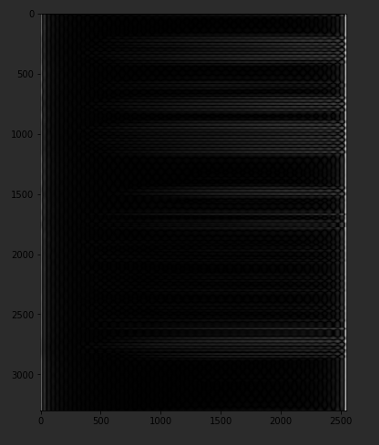
\includegraphics{/Users/christian/Library/Mobile Documents/27N4MQEA55~pro~writer/Documents/6-Thesis/TestDerObjectDetection.png}
\caption{}
\end{figure}

Es zeigte sich außerdem, dass die entsprechenden Algorithmen bei den
Orginal Dokumenten aufgrund ihrere Größe sehr lange brauchen.

Um diese Probleme zu umgehen wurden die Dokumente zunächst geblurred und
kompremiert. Hierzu wurden Bereiche von Pixeln zusammengefasst und auf
einen Durchschnittswert gesetzt. Hierdurch sind die einzelnen Buchstaben
nicht mehr erkennbar, was allerdings für die Erkennung auch nicht
Notwendig ist. Das Ergebnis muss jedoch in Zukunft wieder hochskaliert
werden.

Des weiteren wurde ein Erkennungsfilter erstellt. Da Tabellen eine
einheitliche Struktur haben, kann auch direkt nach ihnen gesucht werden.
\\
Die Struktur einer Tabelle kann dabei in Form einer Sinuskurve mit
folgender Formel abgebildet werden:

\(f(x)=\sin(\frac{x}{b} * 2\pi)\)

Dabei stelt b die länge des Filters, bzw. die Länge der gesuchten Spalte
da. \\
Stellt man sich die Kurve grafisch vor, so stellen die positiven Stellen
den Spalten der Tabelle dar, die negativen den Abstand zur nächsten.

Als Längen werden dabei Bruchteile der Seitenbreite genutzt, z.b. die
Hälfte, ein Drittel oder ein Viertel. Der entsprechenden Filter wird
dann in X und Y Richtung über das Bild geschoben und ein summierter
Zwischenwert von Filter und betrachteter Spalte oder Zeile berechnet.
Daraus ergeben sich zwei Heatmaps, welche wieder kombinieren sind.

\begin{figure}
\centering
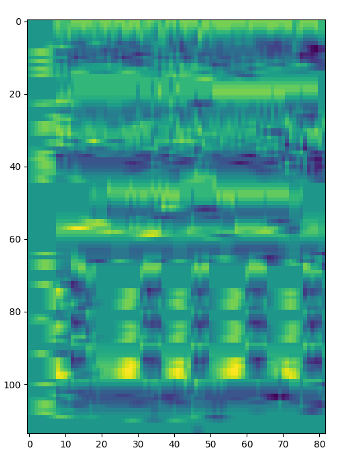
\includegraphics{/Users/christian/Library/Mobile Documents/27N4MQEA55~pro~writer/Documents/6-Thesis/HeatMapinX-Richtung.png}
\caption{}
\end{figure}

\begin{figure}
\centering
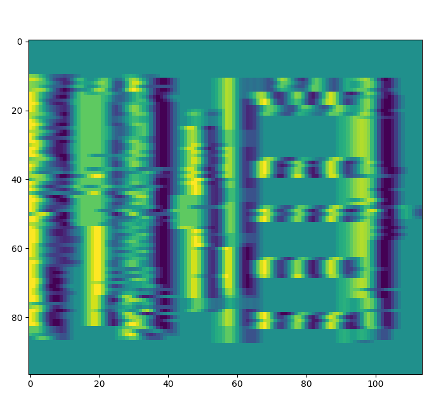
\includegraphics{/Users/christian/Library/Mobile Documents/27N4MQEA55~pro~writer/Documents/6-Thesis/HeatMapiny-Richtung.png}
\caption{}
\end{figure}

Die Stellen an denen beide Heatmaps einen Auschlag markieren, wird nun
in einer Kombination ebenfalls markiert.

\begin{figure}
\centering
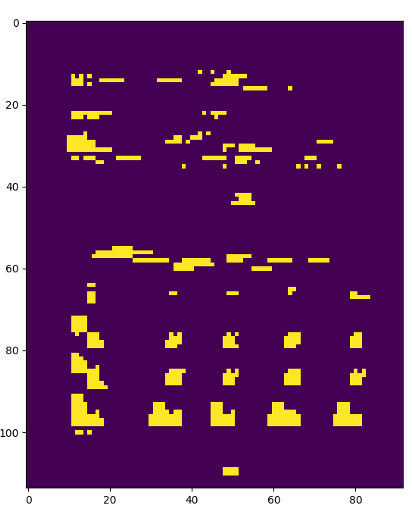
\includegraphics{/Users/christian/Library/Mobile Documents/27N4MQEA55~pro~writer/Documents/6-Thesis/Zielmap.png}
\caption{}
\end{figure}

Im Ergebnis ist die Tabelle noch deutlich erkennbar. Leider weisen
jedoch auch Teile des Textes die gleichen Muster wie eine Tabelle auf,
weswegen Sie auf diesem Bild auch vertreten sind.

Dadurch ist das Ergebnis leider nicht eindeutig, es kann jedoch für
weitere Analysen genutzt werden. \\
Dafür wurden drei Möglichkeiten geplant:

\hypertarget{header-n98}{%
\subparagraph{Ansatz Eins: Verbessern der Filter}\label{header-n98}}

Der erste Ansatz greift beim Erstellen der Filter. Dabei wird ein
Künstliches NN trainiert, welches die Frequenzanalyse der
unterschiedlich langen Filter als Input nimmt, und dann auf Basis der
Änderungen entscheidet welcher Filter am besten geeignet ist. Das Netz
muss dabei mehrere Bilder als Input nutzen können und eine Zahl
ausgeben.

\hypertarget{header-n100}{%
\subparagraph{Ansatz Zwei: Analyse der Heatmap}\label{header-n100}}

In einem zweiten Ansatz wird das entsprechende Bild zunächst mittels
Frequenzanalyse in eine Heatmap umgewandelt. Auf Basis dieser wird dann
ein Neuronales Netz trainiert, welches aus der Kombination die Tabelle
erkennen kann.

\hypertarget{header-n102}{%
\subparagraph{Ansatz drei: Eine Kombination}\label{header-n102}}

Der dritte Ansatz setzt an der gleichen Stelle an wie der erste, soll
jedoch nun die Position der Tabelle ausgeben. Dabei werden die gleichen
Ergebnisse wie zu Beginn in das Netz geladen. Das Netz soll nun jedoch
die veränderten Bilder analysieren und so erkennen, wo sich die Tabelle
befindet.

\hypertarget{header-n104}{%
\paragraph{Einsatz von Neuronalen Netzen}\label{header-n104}}

Aufgrund der zeitlichen Beschränkung wurde nur der zweite Ansatz
umgesetzt.

Für das Training werden dabei Testdaten benötigt. Um die Machbarkeit des
Prinzips festzustellen wurden zunächst synthetische Daten erzeugt. Dabei
wurde das gewünschte Muster mit einer zufälligen Sinuskurve erstellt und
der Hintergrund mit einem Rauschen belegt. Das Netz sollte dabei lernen
nur die Tabelle zu erkennen und das Rauschen nicht zu beachten. \\
Die Testdaten sind dabei zunächst deutlich kleiner im Umfang als die
orginal Dokumente.

\begin{itemize}
\item
  Aufbau des Netzes?
\end{itemize}

\begin{figure}
\centering
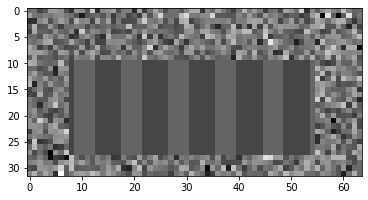
\includegraphics{/Users/christian/Library/Mobile Documents/27N4MQEA55~pro~writer/Documents/6-Thesis/TestBild.png}
\caption{}
\end{figure}

Zunächst wurde das Netz trainiert um eine Maske zu erstellen welche die
Zielfläche markieren sollte. Die ersten Tests zeigten jedoch das das
Netz bei den gegebenen Beispielen als Ergebnis nur eine einfarbige
Fläche ausgibt. Das hier gezeigte Problem wurde zunächst als Overfitting
eingestuft. Gegen diese Einschätzung spricht jedoch, dass das bestehende
Netz die gegebenen Beispiele nicht gelöst hat, sondern nur eine
Minimallösung für das Problem erbrachte. \\
Um diesen Effekt aufzuheben wurden mehrere Tests durchgeführt. Dabei
wurden verschiedene Variablen wie die Learn Rate oder die Anzahl an
zusätzlichen Schichten angepasst, was jedoch nur bedingt zu einer
Verbesserung der Situation führte. Gleichzeitig zeigte sich in allen
Modellen ein gleicher Trainingsverlauf. Dabei stieg die Genauigkeit
während des Trainings an, jedoch gleichzeitig auch der loss Wert. Dieser
beschreibt das Ergebnis der Kostenfunktion und sollte im Verlauf der
Optimierung eigentlich sinken.

Das Netz wurde daher umgebaut, so dass nun direkt Zielkoordinaten
ausgegeben wurden. Dieser Ansatz brachte deutlich bessere Ergebnisse:

\begin{figure}
\centering
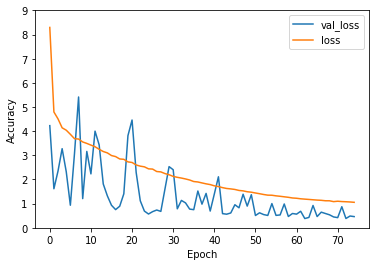
\includegraphics{/Users/christian/Library/Mobile Documents/27N4MQEA55~pro~writer/Documents/6-Thesis/TabellenerkennungTrainingsAuswertung.png}
\caption{}
\end{figure}

In folgendem Beispiel stellt die Gelbe Fläche den gesuchten Bereich dar.
Das Ergebnis des Netzes wird in Rot dargestellt.

\begin{figure}
\centering
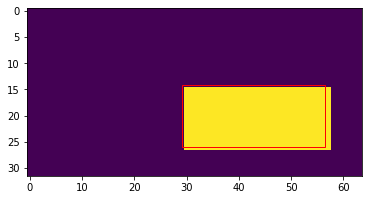
\includegraphics{/Users/christian/Library/Mobile Documents/27N4MQEA55~pro~writer/Documents/6-Thesis/TabellenerkennungTrainingsBeispielBild.png}
\caption{}
\end{figure}

Das Ergebnis ist nicht perfekt, zeigt jedoch das die generelle
Fuktionsweise funktioniert.

Beim Training stellte sich jedoch auch eine Einschränkung herraus: \\
Für eine Nutzung mit den Orginal Dokumenten muss das Netz in seinem
Umfang deutlich vergrößert werden. Dadurch müssen deutlich mehr
Dokumente fürs Training genutzt werden um gleiche Ergebnisse zu
erzielen. Dadurch erhöht sich außerdem der Zeitliche Aufwand den das
Netz zum trainieren benötigt massiv.

Das Netz ist außerdem darauf ausgelegt eine Tabelle zu erkennen. Sollten
mehrere Tabellen auf dem Dokumenten vorhanden sein funktioniert das Netz
nicht mehr wie vorgesehen.

Ein weiteres Problem ist die Zeit welche das System benötigt um ein
Dokument zu verarbeiten. Durch die vorherige Berechnung benötigt das
Netz häufig bis zu einer Minute pro Dokument.

Um diese Probleme zu lösen wurde das Netz neu geplant. Dabei wurde unter
anderem die Aufgabe des Netzes neu bedacht.

\hypertarget{header-n122}{%
\paragraph{PLATZHALTER}\label{header-n122}}

Aufbauend auf den erfolgen des DeepDeSRT wurde das Netz neu entworfen.
Nun soll das Netz nicht mehr erkennen wo die Tabelle ist, sondern ein
gegebenes Bild klassifizieren. Das Prinzip wird dabei in der Object
Detection verwendet.

Dabei werden Bildausschnitte gewählt, welche dann durch ein Neuronales
Netz klassifiziert wird. Dabei gibt das NN eine Wahrscheinlichkeit aus.

Um die Bildausschnitte zu wählen gibt es verschiedene Methoden: Zum
einen kann das gesamte Bild in Ausschnitte unterteilt werden um alle zu
klassifizieren. Durch die Anzahl an möglichen Ausschnitten dauert diese
Methode entsprechend lang.\\
Dies kann verbessert werden, indem man zunächst Bereiche des Bildes mit
ähnlichen Kontouren, Farben oder intensität zusammenfasst und diese dann
Klassifiziert. Dies beschleunigt den Vorgang deutlich.

Einen neuen Ansatz bietet das YOLO Netz

\hypertarget{header-n127}{%
\paragraph{Yolo - You only look once}\label{header-n127}}

Yolo wurde von Joseph Redmon und Ali Farhadi der University of
Washington entwickelt und ist ein völlig neuer Ansatz der Objekt
Erkennung. Dabei wird das Netz nicht mehr in einzelne Teile zerlegt,
sondern durch ein einziges Netz geschickt. Das Netz unterteilt das Bild
dann selbst in Boxen welches es klassifiziert. Durch diese Methode wird
zum einen nur noch ein Netz pro Bild benötigt. Zum anderen ist es laut
Aussage der Entwickler 1000 mal schneller als die herkömlichen Methoden.

Auf Grund dieser Prozess Beschleunigung wurde Yolo als Netz für diese
Arbeit gewählt. Das Netz wurde dabei mit dem PubLayNet Trainingsset
trainiert.

Anders als beim DeepDeSRT wurde das Netz nicht einzig auf Tabellen
ausgelegt, sondern auf alle möglichen Beispiele. Es wurde außerdem auf
die Kompremierung der Bilder verzichtet wodurch nun Dokumente in ihrer
ursprünglichen Größe geladen werden ohne einen Nachteil zu erhalten.

Es wurden folgende Klassifizierungen identifiziert:

\begin{enumerate}
\def\labelenumi{\arabic{enumi}.}
\item
  Text
\item
  Überschrift
\item
  Liste
\item
  Tabelle
\item
  Figur/Grafik
\end{enumerate}

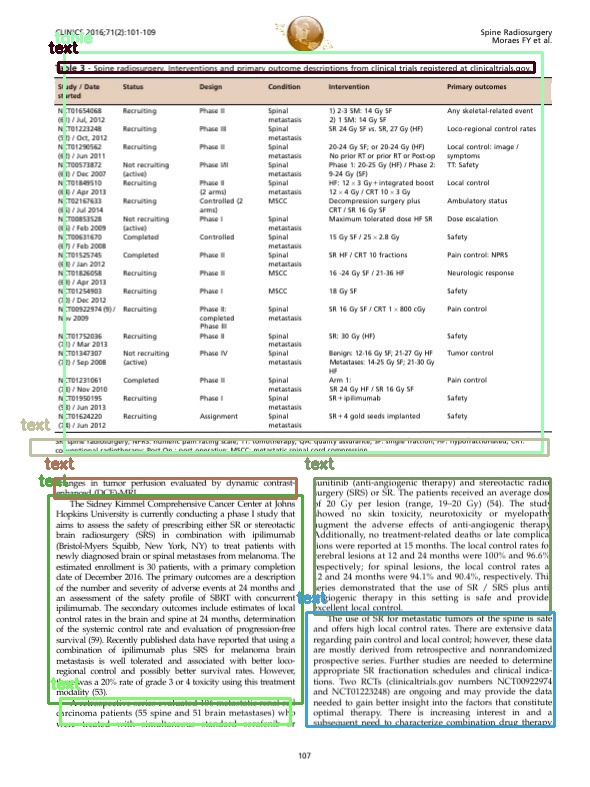
\includegraphics{/Users/christian/Library/Mobile Documents/27N4MQEA55~pro~writer/Documents/6-Thesis/result.jpg}

\hypertarget{header-n144}{%
\paragraph{Ergebnis}\label{header-n144}}

Nach dem Training wurden mehrere Tests mit Beispiel Dokumenten
durchgeführt. Dabei zeigte sich, dass das Netz alle Objekte erkennt,
jedoch die Bereiche nicht perfekt beschreiben kann.

Bei der Nutzung des Netzes fielen noch weitere Effekte auf. \\
Füttert man das Netz mit Dokumenten größerer Pixeldichte so erkennt das
Netz keine Objekte. Eine Theorie hierfür wäre, dass das Netz Pixelgenau
arbeitet. Die entsprechden Objecte sind bei einem Dokument von größere
Pixeldichte jedoch deutlich zu groß um erkannt zu werden. Dieser Umstand
kann jedoch umgangen werden indem das Dokument auf die Größe der
Testdokumente verkleinert wird.

Die Abweichung der Boxen kann durch einen Filter behoben werden. Dieser
würde die Kanten der einzelnen Objecte erkennen und so die Boxen
anpassen. Aufgrund der Zeitlichen Einschränkung der These wurde diese
Optimierung nicht durchgeführt.

Nachdem man die Tabellen nun mit Postionen finden kann, wird ein
weiterer Mechanismus benötigt um die entsprechenden Felder zu finden. Da
Tabellen in ihrem Aussehen und Aufbau sehr unterschiedlich sind, reicht
ein klassischer Algorithmus nicht aus. \\
ALs Lösung für dieses Problem wurde zunächst gepalant das YOLO Netz
erneut einzusetzen, diesmal allerdings darauf trainiert Blöcke von
Zeichen zu finden. Eine Alternative dazu ist die Schrifterkennung.

\hypertarget{header-n149}{%
\subsection{OCR - Optical Character Recognition}\label{header-n149}}

Die Schrifterkennung soll aus der gefundenen Tabelle die Wörter, Zahlen
und Buchstaben extrahieren.

Die entsprechende Technik wurde bereits 1958 zum ersten mal vorgestellt.
Dabei erstellten Frank Rosenblatt und Charles Wightman in Zusammenarbeit
mit dem MIT und dem United States Office of Naval Research das Mark 1
perceptron. Damals noch eher in Form eines physischen Computers als
einer Software, konnte dieses System bereits einfache Ziffern in Bildern
der Maße 20 x 20 Pixeln erkennen. Das zugrundeliegende Verfahren wurde
seitdem immer weiter verbessert, und ist heute ein gut erforschtes Feld
mit vielen verschiedenen Lösungen.

Für dieses Projekt wurden mehrere freie Tools für die Schrifterkennung
getestet. Besonders stachen dabei das Tool Tesseract und die Vision
Library des IOS Systems hervor. Beide sind offline Lösungen.

Tesseract ist eine von Google Entwickelte freie Texterkennungssoftware.
Sie kann Textzeichen und Textzeilen erkennen, sowie Layoutanalysen
durchführen. Dabei beherrscht das Programm mehr als 100 Sprachen, sowie
mehrere verschiedene Schriften wie Chinesisch, Arabisch oder Griechisch.
Nach Aussage eines Test der Zeitschrift c't (QUELLE?) nutzt Google das
Tool selbst für eigene Produkte wie Google Books. Dabei soll das Tool an
ähnliche Erkennungsraten und Verarbeitungsgeschwindigkeiten wie
kommerzielle Tools herankommen. Auf welcher Grundlage diese Aussagen
getroffen wurden oder auf welche Tools sich bezogen wird wird in diesem
Test leider nicht genannt. Für die Nutzung in diesem Projekt sollte die
Leistung dabei jedoch trotzdem ausreichend sein.

In ersten Tests zeigte sich aber auch Einschränkungen des Tools. Zeichen
wie das Doller Zeichen (\$) werden beispielsweise gerne als 5 oder gar
nicht erkannt.

Das Vision Framework des IOS Systems bietet verschiedene Funktionen,
unter anderem eine eigene Texterkennung. Die Implementierung ist dabei
im IOS System standardmäßig vorhanden und für den Einsatz optimiert.

Beide Tools können neben den erkannten Zeichen auch deren Positionen
ausgeben. Mit Hilfe eines einfachen Algorithmus kann daraus wieder die
Ursprungstabelle exportiert werden.

Im Bereich der Schrifterkennung gibt es auch einige online Tools, wie
z.b. Amazon Rekognition oder Googles OCR. Diese sind in der Regel
deutlich treffsicherer als freie Tools, haben jedoch auch entscheidende
Nachteile.

\hypertarget{header-n158}{%
\paragraph{Rechtliche und Technische Betrachtung von Online
Lösungen}\label{header-n158}}

Die zuletzt betrachteten Tools sind Online Services. Dies bedeutet, dass
alle zu verarbeitenden Dokumente zunächst zu einem Server hochgeladen
werden müssen und auf den Servern des Anbieters verarbeitet werden. Dies
bedeutet, dass alle Tools auf eine Online Nutzung ausgelegt werden
müssen und nur mit Verbindung zum Server funktionieren. Dies schränkt
eine Nutzung auf Mobilen Geräten oder in abgeschotteten Intranets ein.

Zusätzlich müssen bei der Verarbeitung von Daten in Deutschland,
abhängig von Art und Schutzbedarf, gewisse Regelungen zur
Informationssicherheit und zum Datenschutz beachtet werden. Das
Bundesamt für Sicherheit in der Informationstechnik (kurz BSI) hat
hierfür Standards erstellt mit denen eine Risikoanalyse durchgeführt
werden kann. Anforderungen und Bewertungen werden dabei in Reihe 2700-x
der ISO Normen beschrieben. \\
In Deutschland gilt ebenfalls noch die Datenschutz-Grundverordnung (kurz
DSGVO). Diese Europäische Richtlinie vereinheitlicht die Regelungen zur
Verarbeitung von personenbezogenen Daten in Europa und beschreibt unter
anderem die Pflichten des Anbieters. Dabei gilt nach Artikel 25 der
DSGVO, dass der Anbieter des Endsystems den Datenschutz im Rahmen seiner
technischen Möglichkeiten umsetzten muss. Was Datenschutz eigentlich
ist, wird dabei genauer in Art. 5 bis 9 beschrieben.

Bei der hier angesprochenen Nutzung von Cloud Diensten werden diese
Regelungen noch erweitert. Dazu steht in Art. 44 DSGVO, dass die
Übertragung von Daten an ein Drittland oder eine internationale
Organisation nur zulässig ist, wenn sichergestellt werden kann, dass die
Bemühungen zum Datenschutz eingehalten werden.

Das BSI hat hierfür den ''Mindeststandart des BSI zur Nutzung externer
Cloud-Dienste'' herausgegeben. Dieser richtet sich nach § 8 Absatz 1
Satz 1 des Gesetztes über das Bundesamt für Sicherheit in der
Informationstechnik (kurz BSIG). Dabei müssen alle Daten in vorgegebene
Kategorien einsortiert werden:

\begin{itemize}
\item
  Kategorie 1: Privat und Dienstgeheimnisse
\item
  Kategorie 2: personenbezogene Daten
\item
  Kategorie 3: Verschlusssachen gemäß allgemeiner Verwaltungsvorschrift
\item
  Kategorie 4: sonstige Daten welche nicht in die vorherigen Kategorien
  einsortiert werden konnten.
\end{itemize}

Je nach Kategorisierung der Daten müssen die Cloud Dienste dann die
Vorgaben des Anforderungskatalog Cloud Computing des BSI (kurz C5)
erfüllen. Darin werden Auswahlprozesse für den Cloud Anbieter, sowie
empfohlene vertragliche Regelungen festgelegt.

Nutzt man nun die Dienste von Amazon oder Google, so werden die
übertragenen Daten dort gespeichert und zur verbesserung der Dienste
genutzt. Da es sich bei beiden um Firmen mit Sitz in den USA handelt,
gelten dabei auch deren Gesetzte. In diesem Fall gilt z.b. der CLOUD
Act, der ``\emph{*Clarifying Lawful Overseas Use of Data Act}'' unter
welchem Firmen mit Sitz in den USA US-Behörden Zugriff auf gespeicherte
Daten gewährleisten muss, selbst wenn die Speicherung nicht in den USA
erfolgt. Der Datenschutz kann hier also nicht ohne weitere Maßnahmen
gewehrleistet werden.

Auf Grundlage dieser Regelungen und neuen Anforderungen an ein
Endsystem, wurde entschieden für diese Arbeit die oben genannten Offline
Tools zu nutzen.

\hypertarget{header-n175}{%
\subsection{Kontext Detektion}\label{header-n175}}

Um die Nutzung der Daten zu vereinfachen wurde eine Kontext Detektion
entwickelt. Diese soll die Art der erkannten Daten erkennen, damit diese
leichter von einem weiteren System wir z.b. Microsoft Excel verarbeitet
werden können.

Dafür wurden 5 Mögliche Klassifizierung der Daten definiert.

\begin{enumerate}
\def\labelenumi{\arabic{enumi}.}
\item
  Zahlen
\item
  Text
\item
  Kommazahl
\item
  Angaben in Prozent
\item
  Physikalisch Angaben
\item
  Adressen
\item
  Datum
\item
  Mix aus mehreren Daten
\end{enumerate}

Um diese Daten zu klassifizieren werden zunächst Eigenschaften der Daten
identifiziert, z.b. Länge des Datensatzes oder die Anwesenheit
bestimmter Zeichen wie Punkte oder Zahlen. \\
Aus diesen lassen sich den oben gennanten Klassifizierungen ebefalls
Eigenschaften zuweisen. Aus dieser Zuweisung lässt sich dann ein
Entscheidungsbaum erstellen welcher die Klassifizierung durchführt.\\
Eine weitere Möglichkeit der Umsetzung besteht durch den Einsatz eines
Neuronalen Netzes. Das Netz fungiert dabei selbst als Entscheidungsbaum,
nur das die Entscheidungen vom Netz berechnet werden.

Beide Methoden haben ihre vor und Nachteile.

Da ein klassischer Entscheidungsbaum mit Hintergrundwissen des
Entwicklers erstellt wird, kann mit sehr wenigen Beispieldaten
gearbeitet werden wohingegen ein NN viele Daten benötigt um daraus zu
lernen. Dabei nutzt das Netz allerdings alle Daten und kann auch
Verbindungen ziehen die ein Mensch nicht in Betracht ziehen würde. Das
Netz kann außerdem deutlich mehr Beispiele in kürzerer Zeit in Betracht
ziehen und durch die interne Gewichtung deulich Präziser werden und sich
an mehr Szenarien anpassen.

In dieser speziellen Anwendung ist die Anzahl von Daten kein Problem.
Zahlen jeglicher Art lassen sich durch Zufallsfunktionen erstellen und
Texte aus Wörtern zusammensetzten. Dabei kann eine Wörterliste des Duden
als Grundlage genutzt werden, so dass alle Wörter an sich auch Sinn
ergeben. \\
Adressen können unterschiedlich zusammengesetzt werden, da z.b. Firmen
eine andere Anschrift haben können als normale Häuser. Hier können
allerdings auch Real Daten aus dem Telefonbuch oder von Google Maps
verwendet werden.

Nachdem die Datenproblematik kein Problem ist, wie verhält sich der
Zeitliche Aufwand?

Das Entsprechende NN kann von einem geübten Entwickler in ca. 15 min
erstellt werden. Das Training mit 50.000 Datensätzen benötigte ca. 1 min
um eine Präzision von 93\% zu erreichen. \\
Ein Entscheidungsbaum muss bei 7 Eigenschaften für diese Anwendung
\(2^7 = 128\) verschiedene Kombinationen erfassen, auswerten und
Programmieren. Die Programierung ist dabei recht einfach umzusetzten,
weswegen hier wegen der vielen Zeilen Code ca. 30 min geplant werden.
Der Aufwand die Kombinationen zu verbinden ist schwer zu schätzen, bei
einem Fall wie diesem sollte es aber nicht alzu schwer sein, weswegen
dafür weitere 30 minuten eingeplant werden.

Der Vergleich wird hierbei stark durch einige Variablen verwässert. So
werden hier Kennwerte genutzt welche vorher von einem Menschen
festgelegt wurden, also schon eine Vorauswahl haben. Außerdem ist das
Training des NN auf einem speziell dafür ausgelegten Server ausgeführt
worden, wodurch die Trainingszeit natürlich deutlich optimiert ist.

\hypertarget{header-n202}{%
\subsubsection{Welcher Ansatz sollte hier also gewählt
werden?}\label{header-n202}}

In diesem Konkreten Fall kann das Neuronale Netz viel Zeit ersparen. Das
Problem ist jedoch auch durch klassische Algorithmen lösbar, welche
gerade in diesem Fall zu einem besseren Ergebnis fürhren.

Die Stärke der Neuronalen Netze ist zwar deutlich jedoch ist dieses
Problem noch zu klein um Sie wircklich zu nutzen.

\hypertarget{header-n205}{%
\subsection{Prototypische Umsetzung}\label{header-n205}}

Um den Einsatz der Theorie in einem realen Szenario zu demonstrieren,
wurde die Pipeline in einem Prototyp umgesetzt. Dieser wurde in Form
einer I-Phone Application ausgearbeitet um einem realen Beispiel
möglichst nah zu kommen.\\
Da sich nicht alle Teile der Pipeline ohne weitere Forschung im IOS
System umsetzten lassen, wurden Teile wie die Tabellen Erkennung durch
das YOLO Netz an eine Server-Applikation ausgelagert.

In der App kann ein Nutzer ein Foto wählen welches dann analysiert wird.
Das Ergebnis wird dann an den Nutzer ausgegeben so dass es exportieren
werden kann.

\hypertarget{header-n208}{%
\paragraph{Server}\label{header-n208}}

Der Server übernimmt hier die Umsetzung des YOLO Netzes, sowie die
Kontext Detektion. Dafür sendet die App ein entsprechendes Bild oder
eine entsprechende Zeichenkette an den Server und erhält eine
entsprechende Antwort.

\hypertarget{header-n210}{%
\subparagraph{Konkrete Umsetzung}\label{header-n210}}

Der Server wurde in Python geschrieben und mittels des Frameworks Flask
und OpenCV unterstützt. Mittels Flask wird dabei eine API erstellt
welche als Schnittstelle fungiert. \\
Erhält das System eine spezifische Nachricht, so führt die Schnittstelle
die entsprechende Logik aus und sendet das Ergebnis in Form eines Bildes
oder eines Strings zurück. \\
Die Logik greift dabei unter anderem auf das Yolo Netz und die Kontext
Detection in Form eines Tensorflow Netzes zurück. Es existieren außerdem
Funktionen, mit denen das Bild aufbereitet werden kann. Sollte das
Dokument z.b. zwar auf dem gegebenen Bild sein, jedoch beispielsweise
auf einem Tisch liegen, so kann eine Kantendetektion genutzt werden um
das Bild entsprechend zuzuschneiden und dem Netz das erkennen zu
erleichtern.

Um die Aufbereitung weiter zu Unterstützen wurden zusätzlich erste Tests
mit einem Netz durchgeführt welches ein zerknittertes Dokument ohne
Knitter neu erstellen kann. Dieses wurde nur Testweise trainiert und
nicht in den Prototypen integriert.

\begin{figure}
\centering
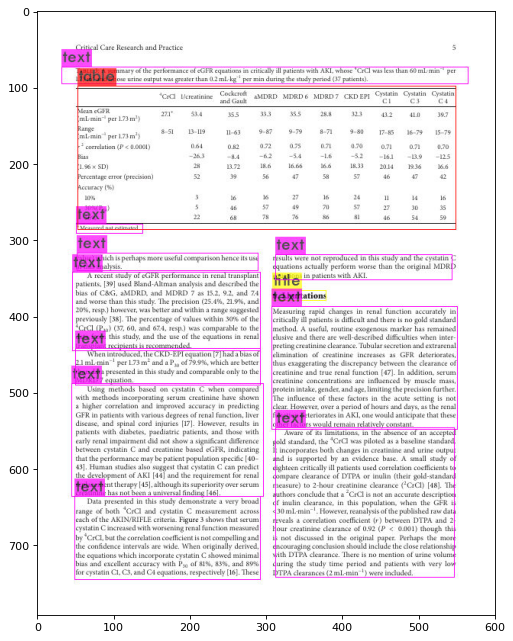
\includegraphics{/Users/christian/Library/Mobile Documents/27N4MQEA55~pro~writer/Documents/6-Thesis/Ergebnis.png}
\caption{}
\end{figure}

Das Program wurde zu Testzwecken auf einem MacBook Air ausgeführt.

\hypertarget{header-n216}{%
\paragraph{App}\label{header-n216}}

Die App wurde komplett in Swift geschrieben. Dabei kann der Nutzer ein
entsprechendes Bild auswählen, welches durch die App analysiert wird. Im
Anschluss kann der Nutzer die Daten exportieren.

Hierzu wird das Bild zunächst an den Server gesendet. Die Antwort wird
dann mit der Hilfe des Vision Framework analysiert und die Textbausteine
werden erkannt.

Da die Textbausteine in keiner spezifischen Reihenfolge ausgegeben
werden wurde ein Algorithmus geschrieben, welcher diese nach Position
sortiert. Im Anschluss kann das Ergebnis ausgegeben werden.

\hypertarget{header-n220}{%
\section{Schluss}\label{header-n220}}

\hypertarget{header-n221}{%
\subsection{Fazit}\label{header-n221}}

Im Rahmen dieser Arbeit wurde ein System erschaffen um Tabellen aus
gegebenen digtalen Dokumenten zu extrahieren und in Daten umzuwandeln.
Dieses System zeigte nicht nur in Tests seine Stärken, sondern auch in
einem funktionierenden Prototyp.

\hypertarget{header-n225}{%
\subsection{Ausblick und Verbesserungen}\label{header-n225}}

Das hier erstellte System ist nicht perfekt. Neben
Optimierungsmöglichkeiten oder zusätzlichen Anwendungen welche in der
Arbeit bereits besprochen wurden, besteht das Problem des zeitlichen
Aufwands welchen das System nun stellt. Eine Möglichkeit der
Beschleunigung besteht hier mit dem Einsatz beser optimierterer Hardware
oder dem Einsatz neuer technischer Methodiken wie Beispielsweise dem
Einsatz eines Quantencomputers.

Ein klassischer Computer rechnet auf Hardware Ebene mit Bits. Dabei
können diese einen Zustand von 0 oder 1 annehmen, woraus sich mittels
Logik Schaltungen erstellen lassen. Quantencomputer nutzen Qubits für
die Berechnung. \\
Ein Qubit nimmt dabei bis zum Zeitpunkt der eigentlichen Abfrage jeden
möglichen Zustand ein, was Superposition gennant wird. Bei einer Abfrage
fällt diese Superposition in sich zusammen und das Qubit nimmt einen
Wert an. \\
Vorstellen lässt sich dies in Form einer kugelförmigen Sphäre mit einem
Vektor im Mittelpunkt. Der Vektor zeigt dabei auf einen Punkt auf der
Sphärenhülle und beschreibt damit die Tendenz des Qubit. Indem wir den
Zeiger nun routieren, verändern wir die Tendenz. Dies können wir mit
Hilfe von Quantum Gates tun. Das Qubit selbst lässt sich also durch die
entsprechende Rotation beschreiben, beziehungsweise mit 4 verschiedenen
Inputs.

Werden nun zwei Qubits genutzt, so beeinflussen sich beide Qubits
gegenseitig, was wiederum neue Effekte bei der Berechnung ergibt.

Diese neue Technologie kann nun zur Entwicklung neuer Netze eingesetzt
werden, genannt Quanten Neuronale Netze oder QNN. Diese Idee wurde zum
ersten mal von Subhash Kak der Oklahoma State University beschrieben. \\
In aktuellen Forschungen lernt das Netz dabei nicht mehr über die
Anpassung von Bias, sondern durch die Anpassung der Quantum Gatter.

Es sei zu beachten, dass der Einsatz eines Quanten Computer nicht
zwangsläufig bedeutet das man das vorhandene Netz beschleunigt. Es ist
eher eine völlig neue Methode zur Erstellung von Netzen.

Um einen Vergleich der neuen Möglichkeiten zu testen, hat das Team
hinter Tensorflow eine Zahlenerkennung in Form eines CNN und eines QNN
erstellt. \\
Um diese Aufgabe weiter zu vereinfachen wurden nur Bilder mit einer 3
und einer 6 genutzt. \\
Um diesen Test nachvollziehen zu können, wurde der Test für diese Arbeit
nachgebaut.

In der ursprünglichen Dokumentation wurde die genutzte Hardware nicht
beschrieben. Da es sich hier jedoch um ein Forschungsteam von Google
handelt, kann davon ausgegangen werden, dass für den Zweck optimierte
Hardware eingesetzt wird.

Die Firma IBM hat Forschern ein weites Netz von Quanten Computern zur
Verfügung gestellt. Darauf kann jeder Forscher mit einem Account seine
eigenen Experimente berechnen lassen. Der Zugang ist dabei jedoch
beschränkt. \\
Für Experimente lassen sich jedoch auch Simulationen nutzen. Diese sind
dabei zwar deutlich langsamer, berechnen jedoch das Optimale Ergebnis
und es treten keine Schmutzeffekte durch äußere Einflüsse auf, was in
praktischen Versuchen durchaus noch der Fall ist. \\
Für die Tests dieser Arbeit wurden Simulatoren genutzt.

Als Trainingsdatenset wurde der MNIST Datensatz verwendet, welcher
Bilder von Zahlen zur Verfügung stellt.

Aus den Ergebnissen des Tests lässt sich nun das CNN und das QNN
gegenüberstellen. Dabei wurden zusätzlich zu den Ergebnissen des Tests
noch die Ergebnisse des Tensorflow Teams betrachtet.

\begin{longtable}[]{@{}lll@{}}
\toprule
& CNN & QNN\tabularnewline
\midrule
\endhead
\textbf{Technische Voraussetzung} & Lässt sich auf jeder CPU ausführen &
Benötigt eine Spezielle Technische Ausstattung\tabularnewline
\textbf{Trainingszeit} & Tensorflow Team: \emph{ca. 3 sec}\textless br
/\textgreater{}eigene Tests: \emph{ca. 33 sec} & Tensorflow Team:
\emph{ca 20 min}\textless br /\textgreater{}eigene Tests: \emph{ca. 4
Stunden und 9 Minuten}\tabularnewline
\textbf{Präzision des Ergebnisses} & Tensorflow Team:
\emph{99\%}\textless br /\textgreater{}eigene Tests: \emph{99\%} &
Tensorflow Team: \emph{85\%}\textless br /\textgreater{}eigene Tests:
\emph{85\%}\tabularnewline
\bottomrule
\end{longtable}

Im direkten Vergleich stellen sich mehrere Unterschiede heraus. Zum
einen lässt sich das QNN nicht ohne weiteres einsetzten, da eine
spezielle Technische Ausstattung benötigt wird, welche häufig nicht zur
Verfügung steht. Zum anderen zeigen die teilweise deutlich besseren
Trainingszeiten des Tensorflow Teams, wie wichtig opimierte Hardware bei
dieser Themaik ist.

Im direkten Vergleich des Netz Ergebnisses ist das CNN dem QNN
überlegen. Nicht nur wird deutlich weniger Zeit benötigt um das Netz zu
trainieren, das Ergebnis ist zusätzlich noch präziser.

Das Grundsätzliche Prinzip des QNN ist jedoch spannend und es ist nicht
auszuschließen das die Technik in Zukunft große Erfolge bringen kann und
dabei völlig neue Netze ermöglicht.

\end{document}
